\documentclass{jsarticle}
\usepackage[top=20truemm,bottom=20truemm,left=25truemm,right=25truemm]{geometry}
\usepackage{amsmath,ascmac,url,amsfonts,bm,here,algorithmic,algorithm,amsthm,color}
\usepackage[dvipdfmx]{graphicx}
\newcommand{\argmax}{\mathop{\rm argmax}\limits}
\newcommand{\argmin}{\mathop{\rm argmin}\limits} 
\newcommand{\expect}{\mathbb{E}} 
\newcommand{\trans}[1]{#1^{\top}}
\newcommand{\pdif}[2]{\frac{\partial#1}{\partial#2}}
\newcommand{\odif}[2]{\frac{\rm{d}#1}{\rm{d}#2}}
\makeatletter
  \def\@maketitle{
  \newpage\null
  \vskip 2em
    \mbox{}\hfill
    \begin{flushleft}
    \textbf{制御システム論分野研究会資料}
    \end{flushleft}
    \begin{flushright}
    {\lineskip .5em
      \begin{tabular}[t]{c}
        \@date \\
        \@author
      \end{tabular}\par}
        \end{flushright}
  \begin{center}
  \let\footnote\thanks
    {\LARGE \@title \par}
    \vskip 1.5em
  \end{center}
    \vskip 1em
  \par}
\makeatother
\title{\large{\bf{進捗報告 9.7}}}
\author{M2 竹内 維吹}
\date{\today}
\begin{document}
\maketitle


\section{前提}
対象のシステムが
\begin{equation}
	\dot{s} = f(s) + g(s)a \label{continuous}
\end{equation}
と書かれており, これを離散化したシステムが
\begin{equation}
	s_{t+1} = f_{d}(s_t) + g_d(s_t)a_t \label{dynamics}
\end{equation}
であるとする. 本研究ではこのような入力アフィン系のセルフトリガー制御を考える. 

\subsection{倒立振子による実験}
倒立時の振子の角度を$\theta=0$とし, 加えられる入力が$A=[-10\textrm{N}\cdot\textrm{m},10\textrm{N}\cdot\textrm{m}]$と制限されるような倒立振子を考える.この倒立振子のダイナミクスは, 以下のように与えられる.
\begin{equation}
	\odif{}{t}\begin{pmatrix}\theta \\ \dot{\theta}\end{pmatrix} = 
		\begin{pmatrix}\dot{\theta} \\ \frac{3g}{2l}\sin{\theta} + \frac{3}{ml^2}a \end{pmatrix} \label{continuous}
\end{equation}

コンピュータで強化学習を行う場合, これを離散化したシステムについて計算を行う必要がある.上記の状態方程式を離散化すると以下のようになる.
\begin{align}
	\theta_{t+1} &= \theta_t+\dot{\theta}_t\delta_t+\frac{3g}{2l}\sin{\theta_t}\delta_t^2+\frac{3}{ml^2}a\delta_t^2 \tag{2a}\\
	\dot{\theta}_{t+1} &=  \dot{\theta}_t+\frac{3g}{2l}\sin{\theta_t}\delta_t+\frac{3}{ml^2}a\delta_t \tag{2b}
\end{align}\label{pend}
\setcounter{equation}{2}
ただし, $\delta_t$は離散化定数であり$\delta_t=0.005$とする.\par


\section{現状確認}
\subsection{セルフトリガー制御}
図\ref{image}のような制御系を考える.
\begin{figure}[h]
	\centering
 	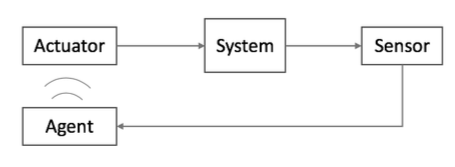
\includegraphics[width=10cm]{event.png}
 	\caption{制御系} \label{image}
\end{figure}\par
これに対するフィードバック制御を考える. 状態変数$s$を観測してアクチュエータに入力信号を送信することを「インタラクション」と呼ぶと,セルフトリガー制御では, 毎時刻インタラクションは行わずに, 次のインタラクションを何ステップ後に行うかをエージェントが決定する. それを数式上で表すため, エージェントの制御則$\pi(s)$は2つの要素からなるベクトル値関数であるとし, 1つ目の要素はアクチュエータに送信する入力$a$,~2つ目の要素は次にインタラクションを行うまでの時間間隔$\tau$を表すものとする.また, 次のインタラクションを行う時刻までは1つ前のインタラクションで送信した入力$a$を加え続けるものとする(ZOH制御).

\subsection{目標点の確認}
研究を通しての目標は「安全性を確保しながら, 最適セルフトリガー制御則$\pi^{*}$の強化学習を実現させること」である。ここで
\begin{align}
	\pi^{*} &= \argmax_{\pi}J(\pi) \\
	J(\pi) &= \expect_{s_0\in d_0}[V^{\pi}(s_0)] \\
	% V^{\pi}(s_0) &= \sum_{i=0}^{\infty} \gamma^i\{-s_i^{\top}Qs_i-\pi_1(s_i)^{\top}R\pi_1(s_i)+\lambda \pi_2(s_i)\} \\
	V^{\pi}(s_0) &= \sum_{i=0}^{\infty} \gamma^i C^{\pi}_i\\
	C^{\pi}_i &= -\int_{T_i}^{T_{i+1}}(s_t^{\top}Qs_t+\tau_ia_i^{\top}Ra_i)\textrm{d}t + \lambda \tau_i, ~T_i = \sum_{l=0}^{i} \tau_l
\end{align}
であり,~$\pi_1, \pi_2$は$\pi$の第1,第2成分である. また, $k$は通しのステップ数, $i$はインタラクションの回数を示し, $a_i, \tau_i$はそれぞれ$i$回目のインタラクションでの方策$\pi$の出力である. \par
以下では方策$\pi$を$\theta$でパラメトライズし, $\theta^{*} = \argmax_{\theta}J(\pi_{\theta})$を解くことによって$\pi^{*} = \argmax_{\pi}J(\pi)$を得るものとする. 方策勾配を用いた強化学習では$\nabla_{\theta}J(\pi)$を用いて$\theta^{*}$を求める. その際方策勾配$\nabla_{\theta}J(\pi)$の近似のため, 実環境とのインタラクションによって得られたデータ組$\{s,a,r,s^{\prime}\}$を用いる. 「学習中の安全」という言葉を, 「このデータ組の収集を決められた安全領域$\mathcal{C}$の内部でのみ行うこと」と定義する.\par


\subsection{実現可能性の検証:サンプル値系での実験}
上記の目標を達成する見込みがあるのかを検証するために, サンプル値系での実験を行う. サンプル値系では,セルフトリガー制御と同様に毎ステップのインタラクションは行わない. セルフトリガー制御との違いは, インタラクションの間隔がエージェントによって状態$s$依存で決定するのではなく, 制御問題の設定として定数$t_{\rm{int}}$で与えられる点である.したがってサンプル値系での制御方策$\pi_{\rm{sample}}$は,アクチュエータに送信する入力信号$a$のみを出力する関数として与える.\par
サンプル値系での実験により, $t_{\rm{int}}=1$のサンプル値系での最適方策
\begin{align}
\begin{cases}
	\pi_{\rm{sample},1} = \argmax_{\pi_{\rm{sample}}} \sum_{i=0}^{\infty} \gamma^i(-s_i^{\top}Qs_i-a_i^{\top}Ra_i) \\
	a_i  = \pi_{\rm{sample}}(s_i)
\end{cases}
\end{align}
を初期方策として,~$t_{\rm{int}}=2$のサンプル値系での最適方策
\begin{align}
\begin{cases}
	\pi_{\rm{sample},2} = \argmax_{\pi_{\rm{sample}}} \sum_{i=0}^{\infty} \gamma^i(-s_i^{\top}Qs_i-a_i^{\top}Ra_i) \\
	a_i  = \begin{cases}
			\pi_{\rm{sample}}(s_i)~(\textrm{if \textit{i} is odd})\\ a_{i-1} (\textrm{otherwise})
		\end{cases}
\end{cases}
\end{align}
 を学習中の安全性を満たしながら学習できるかを検証する. 

\subsection{セルフトリガー制御への発展}
前節での検証によって, インタラクション間隔を大きくしても安全強化学習を行うことが可能であることを確認できたとする. サンプル値系での制御則は入力信号$a$のみを出力する関数であったので, 入力信号$a$とインタラクション間隔$\tau$の二つの要素を出力する必要があるセルフトリガー制御の初期方策として方策$\pi_{\rm{sample},1}$をそのまま用いることはできない. \par
そこで代替策として,
\begin{align}
\begin{cases}
	\pi_1(s)=\pi_{\rm{sample},1}(s)\\
	\pi_2(s)=1
\end{cases}
\end{align}
とする方策$\pi_{\rm{init}}$をセルフトリガー制御の強化学習のための初期方策として用いる.

\subsection{現状持ち合わせているもの}
現在,~$\pi_{\rm{sample},1}$と, その学習プログラムは作成しているが,~$\pi_{\rm{init}}$を作成することはまだできていない. \par
その他, 持っている知識としてCBFとECBF\cite{ECBF}がある. 
 CBFを用いることによって, 状態$s$に対する安全な入力集合を与えることができる.またECBFによって, ZOH制御における, 安全領域を出ないような最大のインタラクション間隔$\tau_{\rm{max}}$を与えることができる.
これらを踏まえて, 今後の研究の道筋を次節に記す.

\section{今後の方針}
\subsection{CBFを用いた安全入力について}
\subsubsection{制御バリア関数(CBF)}
強化学習ではデータの収集に環境とのインタラクションを行う必要がある. DDPGと呼ばれるアルゴリズムは方策オン型の強化学習とよばれ, データの収集方策に学習中の暫定最適方策を用いる. したがって,学習初期の方策では安全性が保証されないことがしばしばある. この課題を解決するために, 制御バリア関数を用いる. \par
関数$h(s)$が以下の条件を満たす時, システム(\ref{continuous})に対する制御バリア関数であるという. 
\begin{equation}
	\sup_{a\in A}\left\{\pdif{h}{s}(f(s)+g(s)a)+K(h(s))\right\} \geq 0 \label{CBF}
\end{equation}
ただし, $K(s)$はクラスK関数である.\par
さて, 2.2節にて登場した安全領域$\mathcal{C}$を
\begin{equation}
	\mathcal{C} = \left\{s \in S~|~h(s)\geq 0\right\}
\end{equation}
として与える. このとき$h(s)$が制御バリア関数であるならば, 状態$s\in C$を初期状態とした時, それ以降の全時刻において, 状態$s$が$s\in C$を満たすようにする入力が存在することを保証する. そのような入力集合は現時刻での状態$s$に依存し,
\begin{equation}
	U(s) = \left\{a \in A~|~\pdif{h}{s}(f(s)+g(s)a)+K(h(s))\geq 0\right\}, \forall s\in C
\end{equation}
としてその集合を与える.\par
学習中の安全性を確保するために, 図2のようにエージェントの出力を$U(s)$の要素に射影するレイヤーを設ける.
\begin{figure}[h]
	\centering
 	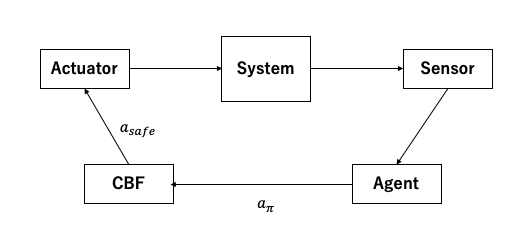
\includegraphics[width=10cm]{barrier_certificate.png}
 	\caption{制御系} \label{cbf}
\end{figure}\\
当面は, エージェントの出力$a_{\pi}$に最も近い$U(s)$の元への射影を考える.


\subsubsection{離散化による影響}
さて, 制御バリア関数による安全性保証は連続システムに対して行われるものであり, コンピュータ上でのシミュレーション環境である(\ref{dynamics})のような離散システムに対しては安全性の保証はできない. つまり,~$\mathcal{C}$の淵の状態に対して, 次ステップでの状態が$\mathcal{C}$を出てしまう可能性があるということである. そこで, 離散化が理由で多少$\mathcal{C}$が出てしまった場合, 最も効率の良い入力(例えば$\theta<0ならa=10$)を用いて, 人為的に$\mathcal{C}$の内部に戻すものとする.\par
また, この問題は制御バリア関数による入力の補償を行う必要がある状況で起こりうるものであるため, その補償が執行されるのを回避するように学習させる方法はないか模索・検証したい. 

\subsection{サンプル値系での検証}
2.3節で記述した通り.

\subsection{セルフトリガー制御の強化学習}
2.4節で記した初期方策$\pi_{\rm{init}}$から, 安全性を保証しながら最適セルフトリガー制御則$\pi^{*}$の学習を試みる. その際, CBFによる安全入力集合への射影に加えて, ECBFによる$\tau$に対する安全性保証も行う. 


\begin{thebibliography}{10}
\bibitem{ECBF}
G. Yang, C. Belta, and R. Tron. “Self-triggered Control for Safety Critical Systems Using Control Barrier Functions."  \textit{In American Control Conference (ACC) Philadelphia, USA}, 2019.
 
 \end{thebibliography}
\end{document}